\section{Nicht ganzzahlige Lösungen}

Wir werden uns zum Abschluss des Kapitels mit der von Aerts und Felsner offen gelassenen Frage beschäftigen, ob die Erkennung von Graphen mit einer SLTR in P liegt -- ob also polynominelle Algorithmen für die Entscheidung existieren, dass für einen gegebenen Graphen eine SLTR existiert. Wie in Abschnitt \ref{dir_multi_flow} erwähnt, impliziert eine nicht ganzzahlige Lösung für ein Gerichtetes-Multi-Fluss-Problem auf einem Graphen mit $n\geq 2$ Paaren von Quellen und Senken, im Allgemeinen nicht die Existenz einer ganzzahligen Lösung und nach Theorem \ref{np_hard} ist die Berechnung einer ganzzahligen Lösung NP-schwer. Die experimellen Ergebnisse aus Kapitel \ref{the_program} lassen jedoch die Möglichkeit offen, dass wir für das betrachtete Netzwerk $\mathcal{N}_G$ die folgende Vermutung beweisen können.

\begin{conjecture}\label{int_conj}
Sei $\tilde{\varphi}=(\tilde{\varphi_1},\tilde{\varphi_2})$ ein nicht ganzzahliger zulässiger Fluss auf $\mathcal{N}_G$, dann existiert auch ein ganzzahliger zulässiger Fluss $\varphi$ und wir können in polynomieller Zeit ein Gutes-FAA aus $\tilde{\varphi_2}$ konstruieren.
\end{conjecture}

\begin{remark}
Wenn wir nicht darauf bestehen, dass ein berechneter zulässiger Fluss auf $\mathcal{N}_G$ ganzzahlig ist, dann lässt sich ein zulässiger Fluss wie in Abschnitt \ref{dir_multi_flow} erwähnt durch lineare Programmierung in polynomineller Zeit finden und das Entscheidungsproblem, ob ein Graph eine SLTR hat läge so in P.
\end{remark}

Es ist uns noch nicht gelungen, einen Beweis von Vermutung \ref{int_conj} zu finden. Wir werden zuerst einen Weg besprechen, um ein FAA aus einer nicht-ganzzahligen Lösung zu konstruieren. Dieses FAA wäre dann nach Vermutung \ref{int_conj} ein Gutes-FAA. Im weiteren Verlauf dieses Abschnittes betrachten wir dann ein Paar der möglichen und verfolgten Beweisansätze. Um die Argumentation einfacher zu gestalten, werden wir das Zwei-Fluss-Problem manchmal als Drei-Fluss Problem, mit einer Lösung $\varphi=(\varphi_s,\varphi_e,\varphi_z)$, betrachten, indem wir Schnyder-, Ecken-, und Zuweisungs-Fluss eigene Typen und somit Quellen und Senken zuweisen.

\begin{proposition}
Sei $\mathcal{N}^*_G$ ein Netzwerk bei dem wir Schnyder-, Ecken-, und Zuweisungs-Fluss jeweils eigene Quellen und Senken zuweisen und das sonst analog zu $\mathcal{N}_G$ konstruiert wird. Dann existiert ein zulässiger (ganzzahliger) Fluss $\varphi^*=(\varphi^*_s,\varphi^*_e,\varphi^*_z)$ auf $\mathcal{N}^*_G$ genau dann, wenn ein zulässiger (ganzzahliger) Fluss $\varphi=(\varphi_1,\varphi_2)$ auf 
$\mathcal{N}_G$ existiert.
\end{proposition}

\begin{proof}
Wir müssen den FAA-Fluss aus $\mathcal{N}_G$ in zwei Typen aufteilen. In der Bemerkung nach Proposition \ref{prop_net_faa} haben wir schon einen Weg beschrieben dies zu tun. In $\mathcal{N}_G^*$ existieren jeweils von der Ecken- und Zuweisungs-Quelle Kanten zum ersten Knoten der Winkeldreiecke. Die Winkel-Senke ist Senke 2 und wir trennen die Dummy-Senke von Senke 2 und machen sie zur Zuweisungs-Senke. Sonst sind $\mathcal{N}_G$ und $\mathcal{N}^*_G$ gleich. Die Bedarfe werden entsprechend aufgeteilt. Somit sind die einzigen von Ecken- und Zuweisungs-Fluss gemeinsam nutzbaren Kanten die ersten Kanten in den Winkeldreiecken. Für den Schnyder-Fluss verändert sich nichts.

Angenommen wir haben einen zulässigen (ganzzahligen) Fluss $\varphi^*=(\varphi^*_s,\varphi^*_e,\varphi^*_z)$ auf $\mathcal{N}_G^*$, dann induziert $(\varphi_s,\varphi_e+\varphi_z)$ auch einen zulässigen (ganzzahligen) Fluss auf $\mathcal{N}_G$. Sei nun $\varphi=(\varphi_1,\varphi_2)$ ein zulässiger (ganzzahliger) Fluss auf $\mathcal{N}_G$. Dann gilt $\varphi_1 = \varphi^*_s$. Wir müssen also $\varphi_2$ aufteilen. Ein (ganzzahliger) FAA-Pfad der ein Winkeldreieck betritt verlässt es entweder durch einen Dummy-Knoten oder führt weiter in das Gebiet. Wir können $\varphi_2$ somit in $\varphi_e^*$ und $\varphi_z^*$ aufteilen. Es bleibt zu zeigen, dass die Bedarfe erfüllt sind. In $\mathcal{N}_G$ führt eine Kante mit Kapazität drei von jedem inneren Gebiet zu Senke 2, die von $\varphi_2$ gesättigt ist. Dieser Anteil des FAA-Flusses wird nach Konstruktion zu $\varphi_e^*$. Somit bleibt in jedem inneren Gebiet $|f|-3$ Zuweisungs-Fluss. Die Bedarfe sind somit erfüllt. Die Ecken-Kompatibilität ergibt sich wie im Beweis zu Theorem \ref{theo_algo}.
\end{proof}

Insbesondere gilt dieser Zusammenhang für eine beliebige Kombination von Ecken-, Schnyder- und Zuweisungs-Fluss zu zwei Flüssen, und wir müssen die Netzwerke nur leicht abwandeln.

\begin{proposition}\label{choose_types}
Für jede beliebige Kombination von Schnyder-, Ecken- und Zu\-weis\-ungs-Fluss als zwei Flüsse auf einem zu $\mathcal{N}^*_G$ analog konstruierten Netzwerk hat existiert ein zulässiger (ganzzahliger) Fluss $\varphi$ genau dann, wenn ein zulässiger (ganzzahliger) Fluss $\varphi^*=(\varphi^*_s,\varphi^*_e,\varphi^*_z)$ auf $\mathcal{N}^*_G$ existiert. Ein zulässiger (ganzzahliger) Fluss $\varphi$ existiert also insbesondere genau dann, wenn eine zulässige (ganzzahlige) Lösung für eine beliebige andere Kombination der Flüsse existiert.
\end{proposition}

\begin{proof}
Wie wir einen zulässigen (ganzzahligen) Fluss $\varphi$ aus $\varphi^*$ konstruieren ist klar. Betrachten wir denn Fall, dass wir Schnyder- und Zu\-weis\-ungs-Fluss zu $\varphi_1$ kombinieren. Wir fügen zwischen der Zuweisungs-Quelle und den Winkeldreiecken für jedes innere Gebiet einen Beutel ein, zu dem eine Kante mit Kapazität $|f|-3$ von der Zuweisungs-Quelle führt (vergleiche Abbildung \ref{pic_faa_choice}). Sei nun $\varphi=(\varphi_1,\varphi_2)$ ein zulässiger (ganzzahlige) Fluss. Für den Zuweisungs-Fluss $\varphi_2=\varphi_z$ verändert sich nichts. Nun bleiben in jedem inneren Gebiet genau drei Winkeldreiecke von $\varphi_z$ ungenutzt. Wir können einen Pfad in $\varphi_1$ Zuweisungs-Fluss oder Schnyder-Fluss zuweisen, indem wir überprüfen, ob er das kleine Quadrat von einem Kanten-Knoten oder einem Winkeldreieck aus betritt. Durch jedes innere Gebiet führen drei Ecken-Pfade und somit $|f|-3$ Schnyder-Pfade. Die Ecken-Kompatibilität erfolgt wieder analog zum Beweis von Theorem \ref{theo_algo}. Die Kombination aus Schnyder- und Ecken-Fluss folgt nach Aerts und Felsner \cite{af15}. Hier reicht wieder der Beutel im Zuweisungs-Fluss um die Korrektheit des Netzwerkes zu erhalten.
\end{proof}

\begin{claim}
Angenommen es existiert eine zulässige nicht-ganzzahlige Lösung $\tilde{\varphi}$ auf $\mathcal{N}_G$ und $\mathcal{N}_G$ lässt keine ganzzahlige Lösung zu, dann müssen die drei Flüsse $\tilde{\varphi}_e, \tilde{\varphi}_z$ und $\tilde{\varphi}_s$ alle nicht-ganzzahlig sein. Insbesondere gilt dies schon auf jedem Teilnetzwerk um ein inneres Gebiet.
\end{claim}

Angenommen nicht, dann könnten wir lokal den ganzzahligen Fluss als Typ 1 und die beiden anderen als Typ 2 definieren. Nach Theorem \ref{theo_int_flow} existiert nun ein zulässiger ganzzahliger Fluss von Typ 2 und wir würden einen ganzzahligen Fluss auf $\mathcal{N}_G$ erhalten. 

Betrachten wir zunächst den zweiten Teil von Vermutung \ref{int_conj}. Die nächste Proposition liefert eine Methode aus einem nicht ganzzahligen zulässigen Fluss ein FAA zu konstruieren.

\begin{proposition}\label{lem_faa}
Sei $\tilde{\varphi}$ ein nicht ganzzahliger zulässiger Fluss auf $\mathcal{N}_G$ und sei $W$ die Menge der vom Zuweisungsfluss $\tilde{\varphi}_z$ genutzten inneren Winkel von $G$. Dann existiert eine Teilmenge $\phi\subseteq W$, sodass aus jedem Gebiet $f$ genau $|f|-3$ Winkel in $\phi$ enthalten sind und in der jeder Knoten $v$ höchstens einmal vorkommt. $\phi$ ist also ein FAA auf $G$.
\end{proposition}

\begin{proof}
Sei $\tilde{\varphi}$ ein nicht ganzzahliger zulässiger Fluss auf $\mathcal{N}_G$. Wir definieren das gerichtete Netzwerk $\mathcal{F}_z$ mit Quelle $s$ und Senke $t$, einem Beutel $B_f$ für jedes innere Gebiet $f$, einem Knoten für jeden inneren Winkel $(f,v) \in W$ und einem Knoten für jeden Dummy-Knoten. Zuerst fügen Kanten mit Kapazität $|f|-3$ von der Quelle zu jedem Beutel ein. Dann folgen Kanten von den Beuteln $B_f$ zu den Winkeln von $f$, von den Winkeln $(f,v)$ zu den Dummy-Knoten $v^*$ und zuletzt eine Kante von jedem Dummy-Knoten zu Senke, jeweils mit Kapazität 1. Die Kanten zu den Beuteln bilden einen Schnitt mit Kapazität $\sum_{f \in F_{in}}(|f|-3)$ und $\tilde{\varphi}_z$ induziert einen zulässigen nicht-ganzzahligen Fluss $\varphi^*$ auf $\mathcal{F}_z$. Die Stärke eines maximalen $s$-$t$-Fluss in $\mathcal{F}_z$ ist somit $\sum_{f \in F_{in}}(|f|-3)$. Nach Theorem \ref{theo_int_flow} existiert also ein ganzzahliger zulässiger Fluss $\varphi$ auf $\mathcal{F}_z$, mit $|\varphi| = |\varphi^*| = |\tilde{\varphi}_z| = \sum_{f \in F_{in}}(|f|-3).$

\begin{figure}
	\centering
  	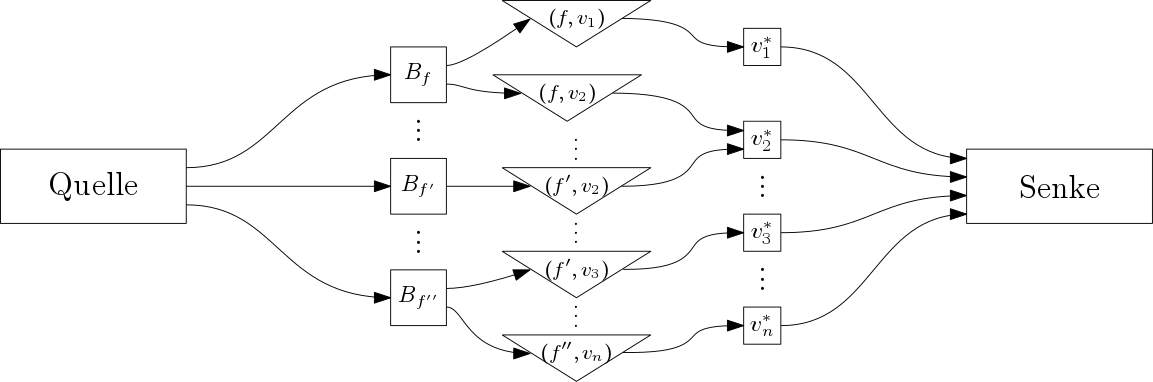
\includegraphics[width=0.9\textwidth]{lem_faa_choice.png}
  	\caption{Skizze des Netzwerkes $\mathcal{F}_z$. Die Kanten von der Quelle zu einem Beutel $B_f$ hat Kapazität $|f|-3$ und alle anderen haben Kapazität 1.}
	\label{pic_faa_choice}
\end{figure}

$\varphi$ weißt nun jedem inneren Gebiet $f$ genau $|f|-3$ Winkel zu und jeder Knoten $v$ kann nur einmal zugewiesen werden. Wenn wir noch die per Konstruktion von $\mathcal{N}_G$ zugewiesenen Knoten am äußeren Gebiet hinzunehmen, dann erhalten wir ein FAA auf $G$.
\end{proof}

Wenn wir zeigen könnten, dass ein wie in Proposition \ref{lem_faa} konstruiertes $\phi$ ein Gutes-FAA ist, folgt Vermutung \ref{int_conj}, da die Existenz eines Guten-FAAs $\phi$ nach Theorem \ref{theo_algo} auch die Existenz eines ganzzahligen zulässigen Flusses $\varphi$ für $\mathcal{N}_G$ impliziert. Die Ergebnisse aus Kapitel \ref{the_program} legen nahe, dass es sich um ein Gutes-FAA handelt. Formulieren wir dies als eine zweite Vermutung.

\begin{conjecture}\label{conj_faa}
Ein wie in Proposition \ref{lem_faa}, aus einem zulässigen Fluss auf $\mathcal{N}_G$ konstruiertes FAA $\phi$ ist ein Gutes-FAA von $G$ und induziert somit eine SLTR.
\end{conjecture}

\begin{example}
Es ist uns nicht möglich mit beliebigen Winkeln aus $W$ zu beginnen und Schritt für Schritt für jedes Gebiet $|f|-3$ Winkel wählen. Betrachte den planaren Graphen $G$ aus Abbildung \ref{lem_faa_choice_ex}. Die beiden SLTRs auf der linken Seite haben die selben Aufhängungen, implizieren jedoch andere FAAs somit auch andere zulässige ganzzahlige Flüsse auf $\mathcal{N}_G$. Seien $\varphi$ und $\varphi'$ diese Flüsse und $f_{r},f_{g}$ und $f_b$ die drei eingefärbten Gebiete. Betrachten wir die Zuweisungs-Flüsse $\varphi_z$ und $\varphi'_z$. Dann gilt $$|\varphi_z(f_r,v)|=|\varphi_z(f_r,u)|=|\varphi_z(f_b,w)| = |\varphi_z(f_g,x)| = 1$$
$$|\varphi_z(f_r,v)|=|\varphi_z(f_r,w)|=|\varphi_z(f_b,u)| = |\varphi_z(f_g,x)| = 1.$$
Der Fluss $\tilde{\varphi}=\frac{\varphi+\varphi'}{2}$ ist ebenfalls zulässig und es folgt:
$$|\tilde{\varphi}_z(f_r,v)|=|\tilde{\varphi}_z(f_g,x)| = 1 \text{ und } |\tilde{\varphi}_z(f_r,w)|=|\tilde{\varphi}_z(f_r,u)| = |\tilde{\varphi}_z(f_b,w)|=|\tilde{\varphi}_z(f_b,u)| = \frac{1}{2}.$$
Somit liegen all diese Winkel in W. Wir können allerdings nicht einfach beginnen in einem Gebiet die benötigte Anzahl an Winkel auszuwählen. In Abbildung \ref{lem_faa_choice_ex} führt dies auf der rechten Seite zu keinem FAA und somit auch zu keiner SLTR. Die Konstruktion des Netzwerkes im Beweis von Proposition \ref{lem_faa} ist somit sinnvoll.

\begin{figure}[h]
	\centering
  	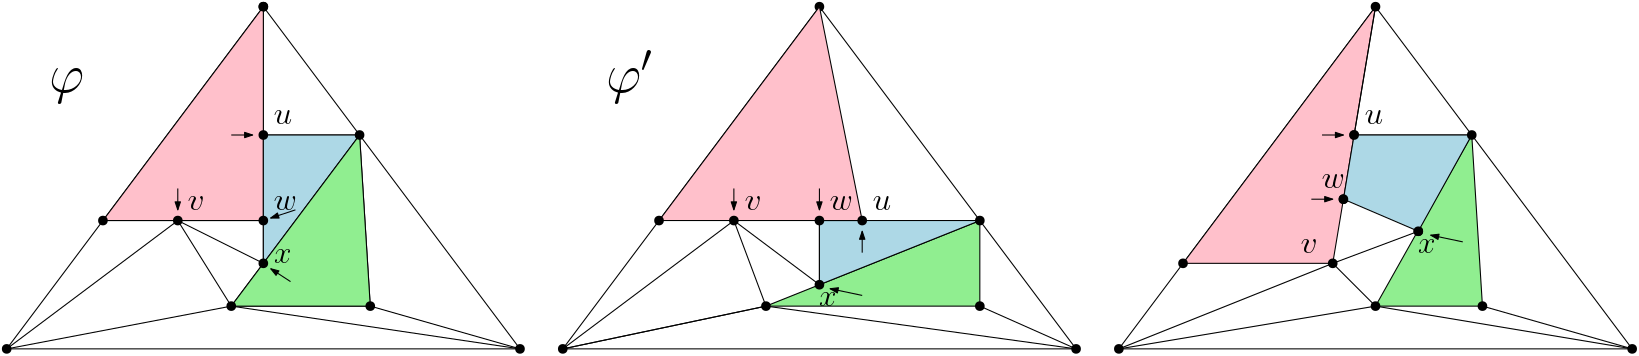
\includegraphics[width=1\textwidth]{lem_faa_choice_ex.png}
  	\caption{Bei der Auswahl der Winkel aus W ist Vorsicht geboten.}
	\label{lem_faa_choice_ex}
\end{figure}
\end{example}

\subsection{Minimale Schnitte in $\mathcal{N}_G$}

Wir wollen in diesem Abschnitt einen ersten möglichen Beweisansatz von Vermutung \ref{int_conj} besprechen. Die Idee ist, dass wir unter der Annahme das nur eine nicht-ganzzahlige Lösung existiert einen minimalen Schnitt in einem Teilnetzwerk von $\mathcal{N}_G$ erzeugen würden, und so zu einem Widerspruch gelangen. 

Angenommen, es existiert ein Netzwerk $\mathcal{N}_G$, für das nur eine nicht ganzzahlige Lösung existiert. Sei $\tilde{\varphi}$ dieser nicht ganzzahlige zulässige Fluss und $\phi$ ein wie in Proposition \ref{lem_faa} aus $\tilde{\varphi}$ konstruiertes FAA für $G$. Sei $\varphi_z$ der eindeutige Zuweisungs-Fluss der dieses FAA auf $\mathcal{N}_G$ kodiert und $\overline{\mathcal{N}}_G$, ein Teilnetzwerk von $\mathcal{N}_G$, aus welchem alle Kanten, die von $\varphi_z$ ausgelastet sind, gelöscht wurden. Die Bedarfe sind weiterhin $|E_{in}|$ und $3|F_{in}|$ für den Schnyder- und Ecken-Fluss. Nach Proposition \ref{choose_types} können wir $\varphi_s$ und $\varphi_e$ zusammenfassen und mit $\varphi_1$ bezeichnen. Wir suchen also nach einem zulässigem ganzzahligem Fluss $\varphi_1 = \varphi_s + \varphi_e$ auf $\overline{\mathcal{N}}_G$ mit Bedarf $|E_{in}| + 3|F_{in}|$, da dann auch eine ganzzahlige Lösung $(\varphi_s,\varphi_e)$ folgen würde. Wir hätten somit einen ganzzahligen Fluss auf $\mathcal{N}_G$ konstruiert, was zu einem Widerspruch führt.

Nach dem Max-Flow Min-Cut Theorem existiert ein zulässiger Fluss auf $\overline{\mathcal{N}}_G$ genau dann, wenn es keinen (Kanten-)Schnitt in $\overline{\mathcal{N}}_G$ mit Kapazität kleiner als $|E_{in}| + 3|F_{in}|$ gibt. Bevor wir fortfahren wollen wir einige Kantentypen aus $\mathcal{N}_G$ benennen.

\begin{itemize}
\item $E_\triangle = $ Die äußeren Kanten in den Winkeldreiecken.
\item $E_\triangledown = $ Die inneren Kanten in den Winkeldreiecken.
\item $S_* =$ Die Kanten von den Dummy-Knoten zur Dummy-Senke.
\item $V_* = $ Die Kanten von den Winkeldreiecken zu den Dummy-Knoten.
\item $E_{\to} = $ Die Kanten von Quelle 1 zu den Kanten-Knoten.
\item $F_\square = $ Die Kanten von den kleinen Quadraten zu inneren Gebieten $f$.
\item $V_{\to} = $ Die Kanten von den Knoten-Knoten zu Senke 1.
\item $e_{d} = $ Die Kante von der Dummy-Senke zu Senke 2
\end{itemize}

Sowohl $\mathcal{S}_1 = E_\triangle \cup E_{\to}$, als auch $\mathcal{S}_2 = F_\square \cup V_{\to} \cup \{e_{d}\}$ sind minimale Schnitte in $\mathcal{N}_G$. Für beide Menge gilt $|\mathcal{S}_1| = |\mathcal{S}_2| = |E_{in}| + \sum{f \in F_{in}}$ und sie trennen die Quellen ($\mathcal{S}_1$) bzw. die Senken ($\mathcal{S}_2$) vom Rest des Netzwerkes ab. Wenn wir nur von den Kanten aus $E_\triangle$, die in $\overline{\mathcal{N}}_G$ übrig sind, sprechen, schreiben wir $\overline{E}_\triangle$. Für die, zu diesen korrespondierenden Kanten im inneren ihrer Winkeldreiecke, schreiben wir $\overline{E}_\triangledown$. Für die Teilmengen von $V_*$ und $S_*$ in $\overline{\mathcal{N}}_G$ schreiben wir $\overline{S}_*$ und $\overline{V}_*$. Die restlichen Mengen sind vollständig in $\overline{\mathcal{N}}_G$ enthalten.

Seien $E_z$ die von $\varphi_z$ genutzen Kanten, die wir aus $\mathcal{N}_G$ entfernen. Dann folgt $|\mathcal{S}_1 \cap E_z| = |E_\triangle \cap E_z| = |\varphi_z|$. Somit ist $\overline{\mathcal{S}}_1 = \mathcal{S}_1 \backslash E_z = \overline{E}_\triangle \cup E_\to$ ein Schnitt in $\overline{\mathcal{N}}_G$. Analog ist $\overline{\mathcal{S}}_2 = F_\square \cup V_{\to}$ ein Schnitt. Für die Kapazität von $\overline{\mathcal{S}}_1$ können wir folgern 
$$ c(\overline{\mathcal{S}}_1) = c(\overline{E}_\triangle) + c(E_\to) = c(E_\triangle) - |\varphi_z| + c(E_\to) = 3|F_{in}| + |E_{in}|,$$
und wieder folgt analog $c(\overline{\mathcal{S}}_2) = 3|F_{in}| + |E_{in}|$.

Falls es sich hierbei um minimale Schnitte handelt, dann würde dies bedeuten, dass eine ganzzahlige Lösung für $\overline{\mathcal{N}}_G$ existiert, mit deren Hilfe wir, zusammen mit $\varphi_z$, eine ganzzahlige zulässige Lösung für $\mathcal{N}_G$ konstruieren könnten, was wiederum ein Widerspruch zu unserer Annahme wäre. Es muss also einen kleineren Schnitt $\mathcal{S}_{min}$, mit $|\mathcal{S}_{min}| \leq 3|F_{in}| + |E_{in}| - 1$, geben. 

\begin{remark}
Falls wir nach dem selben Schema die Kanten aus $\mathcal{N}_G$ entfernen, welche von einem Zuweisungs-Fluss gesättigt sind, der einem FAA entspricht, das keine SLTR induziert, dann muss so ein minimaler Schnitt $\mathcal{S}_{min}$ existieren. Sonst würde ein Widerspruch zu Theorem \ref{theo_ccc} entstehen.
\end{remark}

Falls Vermutung \ref{int_conj} stimmt, dann existiert ist dies nicht zwangsläufig $\mathcal{S}_{min}$ und falls Vermutung \ref{conj_faa} Korrekt ist, dann kann so ein Schnitt nicht existieren. Nehmen wir jedoch für den Moment an, das $\mathcal{S}_{min}$ wie oben beschrieben existiert, dann können wir die folgenden Beobachtungen festhalten.

\begin{claim} \label{cut_types1}
Falls $\mathcal{S}_{min}$ existiert, dann muss auch ein minimaler Schnitt $\mathcal{S}_{min}^*$ in $\overline{\mathcal{N}}_G$ existieren, sodass er nur Kanten von einem der vier Typen $\overline{E}_\triangledown, F_\square, V_\to$ und $E_\to$ enthält.
\end{claim}

\begin{figure}
	\centering
  	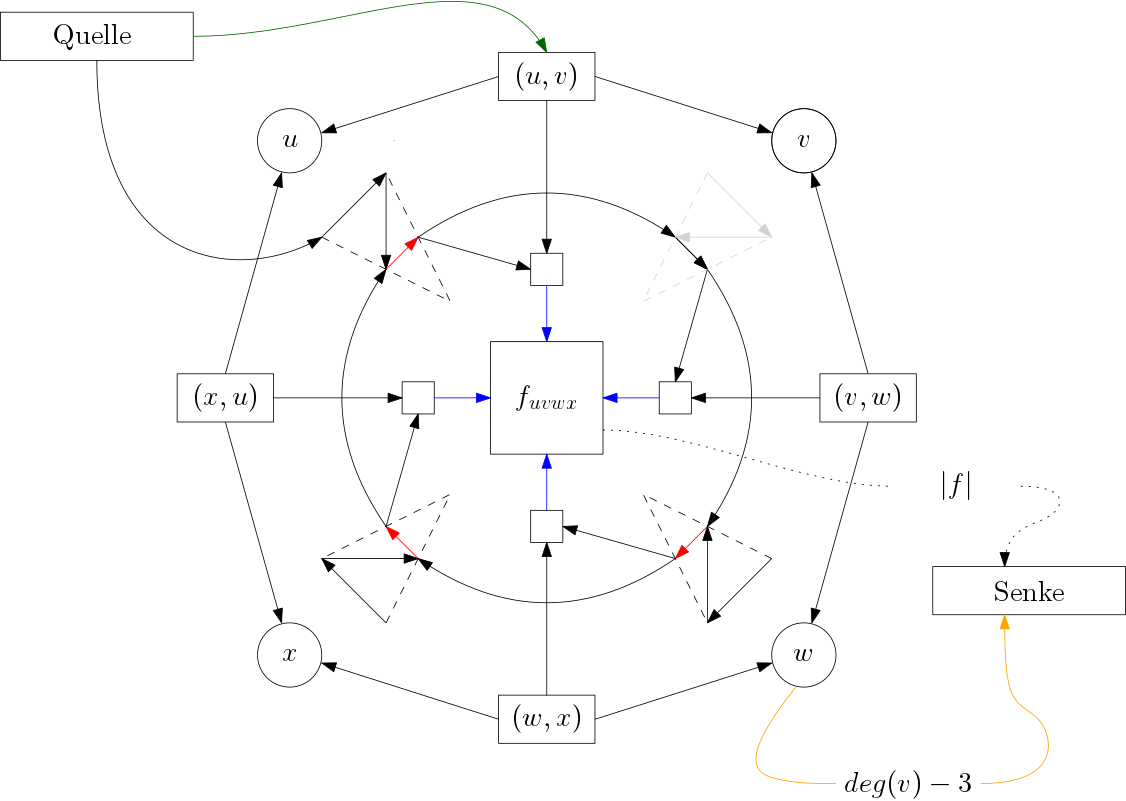
\includegraphics[width=0.8\textwidth]{face_cut.png}
  	\caption{Die vier Kantentypen $\overline{E}_\triangledown$ (rot), $F_\square$ (blau), $V_\to$ (orange) und $E_\to$ (grün) aus denen sich, nach Behauptungen \ref{cut_types1} und \ref{cut_types2}, ein minimaler Schnitt in $\overline{\mathcal{N}}_G$ zusammensetzen müsste.}
	\label{cut_edges}
\end{figure}

Betrachten wir die Kanten in $\mathcal{S}_{min}$. Die vier Kantentypen sind in Abbildung \ref{cut_edges} eingezeichnet. auf einem Pfad von der Quelle bis zu einer Kante in $\overline{E}_\triangledown$, können in $\mathcal{S}_{min}^*$ durch diese ersetzt werden. Ebenso können Kanten zwischen zwei Winkeldreiecken, oder von einem Winkeldreieck zu einem kleinen Quadrat in $\mathcal{S}_{min}^*$ durch die entgegen dem Uhrzeigersinn nächste Kante in $\overline{E}_\triangledown$ ersetzt werden. Kanten zwischen einem Kanten-Knoten und einem Knoten-Knoten, oder einem kleinen Quadrat, können in $\mathcal{S}_{min}^*$ durch eine Kante in $E_\to$ ersetzt werden. Abschliessend können Kanten, von einem inneren Gebiet zu Senke in $\mathcal{S}_{min}^*$ ,durch das hinzufügen von allen Kanten aus $F_\square$ an diesem Gebiet, ersetzt werden.

\begin{claim}\label{cut_types2}
Falls $\mathcal{S}_{min}$ existiert, dann muss auch ein minimaler Schnitt $\mathcal{S}_{min}^*$ in $\overline{\mathcal{N}}_G$ existieren, sodass er nur Kanten von einem der vier Typen $\overline{E}_\triangledown, F_\square, V_\to$ und $E_\to$ enthält. Er enthält aus jeder der Mengen $\overline{E}_\triangledown, F_\square, V_\to$ und $E_\to$ mindestens eine, aber aus keiner der Mengen alle Kanten.
\end{claim}

\begin{proof}
Falls ein solcher ein Schnitt $\mathcal{S}_{min}^*$ existiert, dann kann $\mathcal{S}_{min}^*$ nicht alle Kanten $\overline{E}_\triangledown$ enthalten. Sonst könnten wir aus $\mathcal{S}^*_{min} \cup (E_\triangle \cap E_z)$ einen Schnitt $\mathcal{S}$ mit der gleichen Kapazität konstruieren, indem wir die Kanten $E_\triangledown \cap \mathcal{S}^*_{min}$ durch die Korrespondierenden Kanten in $E_\triangle$ ersetzen. Es folgt $\mathcal{S} \supseteq\mathcal{S}_1$, was ein Widerspruch ist. Falls $\mathcal{S}_{min}^*$ jedoch keine Kante aus $\overline{E}_\triangledown$ enthält, dann muss $\mathcal{S}_{min}^*$ alle Kanten aus $F_\square$ enthalten, weil $\mathcal{S}_{min}^*$ ein Schnitt ist. Falls $\mathcal{S}_{min}^*$ alle Kanten aus $F_\square$ enthält, dann können wir annehmen, dass $\mathcal{S}_{min}^*$ auch alle Kanten aus $V_\to$ enthält. Es folgt $\mathcal{S}^*_{min} \cup \{e_d\} \supseteq \mathcal{S}_2$, was erneut einen Widerspruch bedeutet. Angenommen er enthält keine Kante aus $F_\square$, dann muss er alle Kanten aus $\overline{E}_\triangledown$ und $E_\to$ enthalten und es würde $\mathcal{S}^*_{min} \cup (E_\triangle \cap E_z)$ wäre wie oben erneut ein Schnitt mit Kapazität $\geq |\mathcal{S}_1|$. 

Es bleibt die Mengen $E_\to$ und $V_\to$ zu betrachten. Aus $\mathcal{S}_{min}^*\cap E_\to = \emptyset $ folgt $F_\square\subseteq\mathcal{S}_{min}^*$ und aus $\mathcal{S}_{min}^*\cap V_\to = \emptyset $ folgt $E_\to \subset  \mathcal{S}_{min}^*$. Im Fall $E_\to \subset  \mathcal{S}_{min}^*$ brauchen wir in jedem inneren Gebiet mindestens drei Kanten in $\mathcal{S}_{min}^*$, womit wir wieder mindestens Kardinalität $|S_1|$ erreichen. Wir betrachten als letztens $V_\to$. Hierbei ist zu beachten, dass für Knoten $v$ mit deg$(v) \leq 3$ keine Kante in $\mathcal{N}_G$ existiert. Es gelte $V_\to \subset  \mathcal{S}_{min}^*$, dann muss $\mathcal{N}_G$ noch mindesten $|E_\to|-|V_\to|$ Kanten enthalten, um den Schnyder-Fluss zu unterbrechen, was ein Widerspruch ist. Gelte nun $\mathcal{S}_{min}^*\cap V_\to = \emptyset$. Wir benötigen erneut mindestens $|E_{in}|$ Kanten in $\mathcal{S}_{min}^*$ um den Schnyder-Fluss zu unterbrechen und erhalten somit einen letzten Widerspruch. Behauptung \ref{cut_types2} ist somit richtig.
\end{proof}

Schnyder- und Ecken-Fluss in $\overline{\mathcal{N}}_G$ können nur über die Kanten von Typ $E_\to, V_\to$ und $F_\square$ beziehungsweise $\overline{E}_\triangledown$ und $F_\square$ fließen. Der einzige Kantentyp der in beiden vorkommt ist $F_\square$. Wir finden genau dann keinen ganzzahligen Fluss auf $\overline{\mathcal{N}}_G$, wenn es keinen Ecken-Kompatiblen Schnyder-Wood $\sigma$ zu $\phi$ gibt. Somit muss jeder zulässige Schnyder-Fluss in mindestens einem Gebiet die kleinen Quadrate so auslasten, dass es aus mindestens einem freien Winkel keinen Ecken-Pfad geben kann. Alle kleinen Quadrate zwischen einem freien Winkel und dem im Uhrzeigersinn nächsten müssen somit vom Schnyder-Fluss gesättigt sein. So ein kleines Quadrat ist in Abbildung \ref{combined_face_not_corner}) rot eingefärbt. Wir nennen die Kante an einem kleinen Quadrat ein \textit{blockierendes} Quadrat, falls ein zulässiger Schnyder-Fluss existiert, sodass an diesem kleinen Quadrat ein Widerspruch zur Ecken Kompatibilität auftritt.

\begin{claim}
Falls $\mathcal{S}_{min}$ existiert, dann existiert ein Schnitt $\mathcal{S}^*_{min}$ wie in Behauptung \ref{cut_types2}, welcher alle blockierenden Quadrate enthält.
\end{claim}

Falls ein blockierenden Quadrat nicht in $\mathcal{S}^*_{min}$ enthalten ist, enthält $\mathcal{S}^*_{min}$ die korrespondierenden Kanten aus $E_\to$ und die gegen den Uhrzeigersinn nächste Kante aus $E_\triangledown$. Da es sich um ein blockierendes Quadrat handelt kann der Ecken-Fluss aus diesem Winkeldreieck nicht vorher das Gebiet verlassen. Wir können somit die Kante am Winkeldreieck in $\mathcal{S}^*_{min}$ durch das blockierende Quadrat ersetzen.

\begin{figure}
	\centering
  	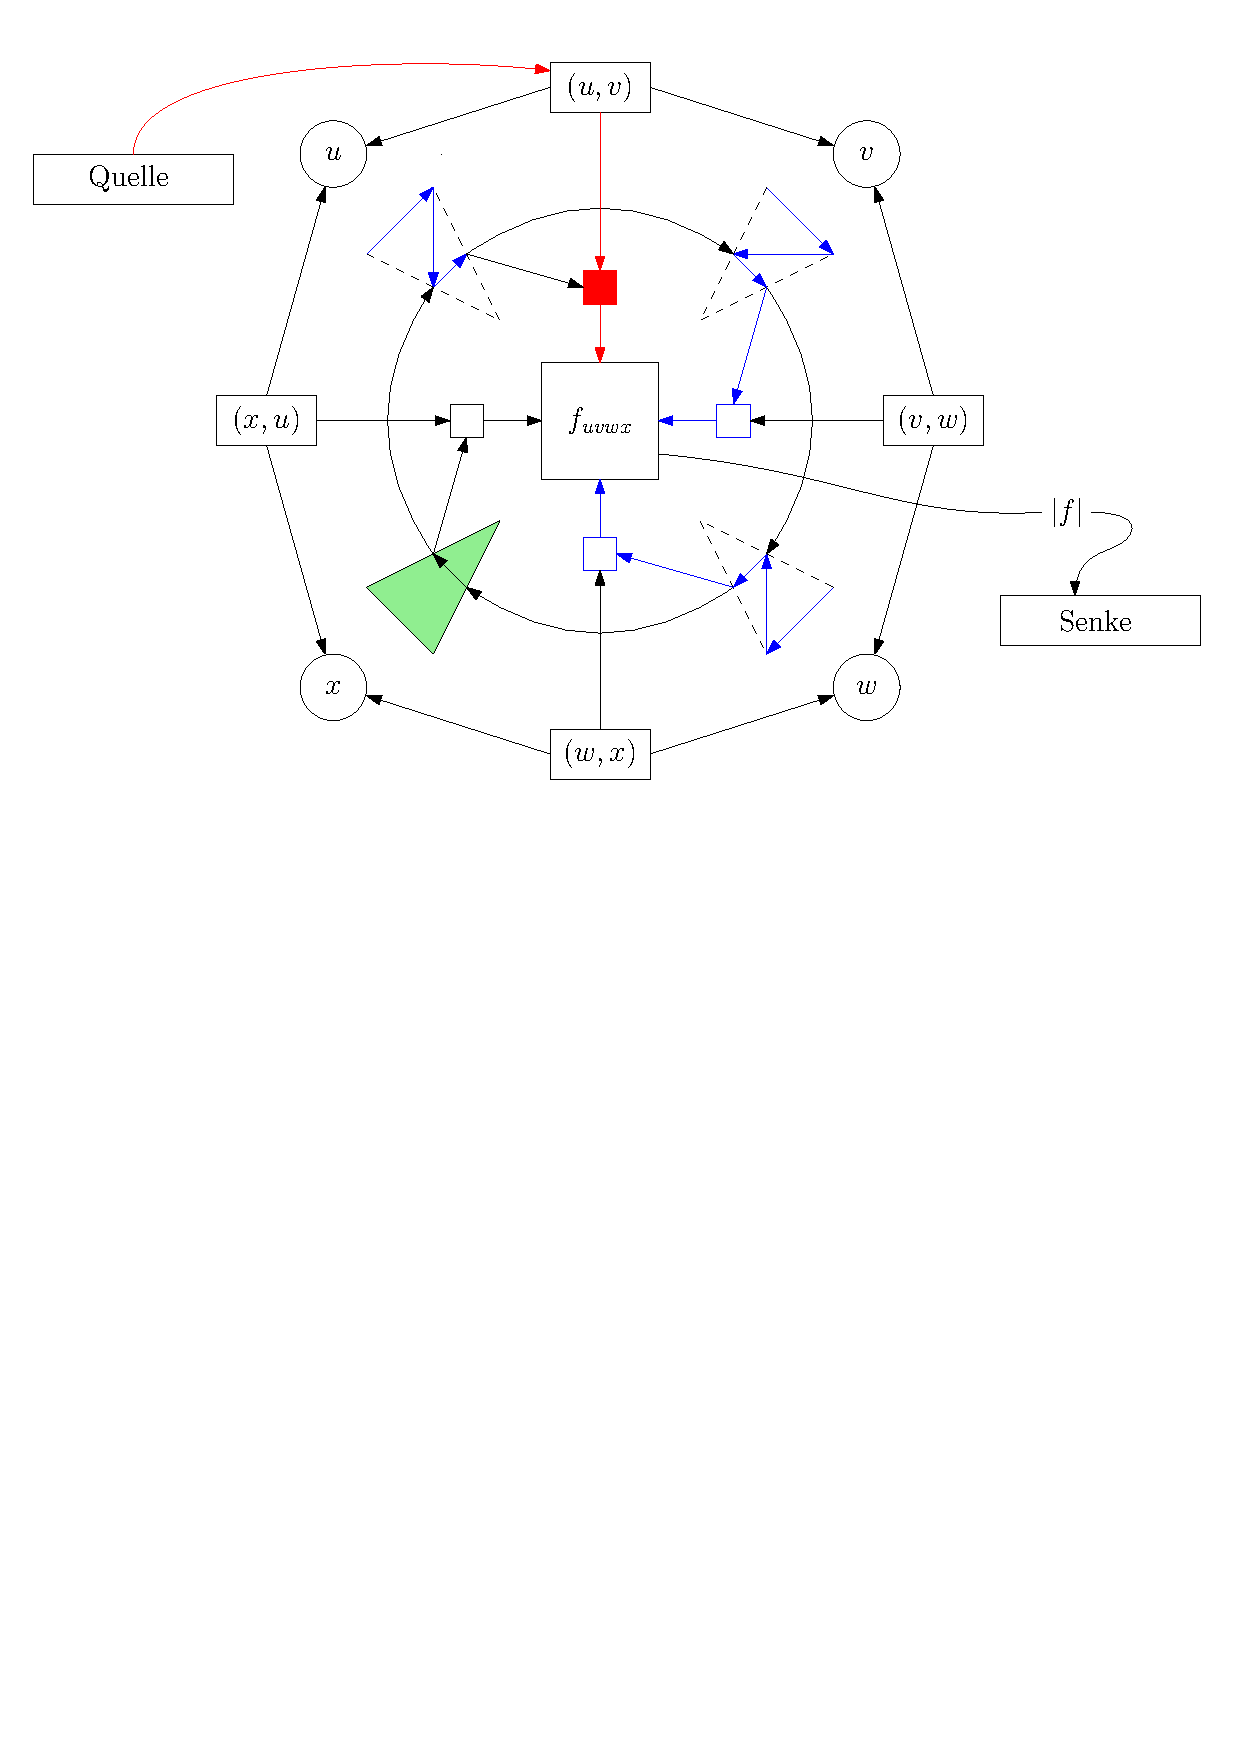
\includegraphics[width=0.8\textwidth]{combined_face_not_corner.pdf}
  	\caption{Der Schnyder-Fluss (rot) ist nicht Ecken kompatibel zum FAA $\phi$ (grün). Somit muss ein blockiertes Quadrat (hier in rot) in $\mathcal{N}_G$ existieren und durch mindestens einen freien Winkel kann kein Ecken-Pfad führen.}
	\label{combined_face_not_corner}
\end{figure}

